\chapter[Campos Finitos (Finite Fields)]{Campos Finitos (Finite Fields)} \label{teo:filds}

Uma noção básica de um campo finito pode ser explicitada como um conjunto que possui um número finito de elementos. Neste, define-se 2 operações, normalmente adição e multiplicação, possuindo as seguintes propriedades para qualquer campo $F$:

\begin{itemize}
	\item Para qualquer elemento $a$,$b$ dentro de um conjunto $F$, as operações de adição e multiplicação são operações binárias em $F$.
	\item Para qualquer elemento dentro do conjunto $F$ as propriedades associativas e distributivas devem serem mantidas. 
	\item Para qualquer $a$,$b$ em $F$, as seguintes relações são mantidas: $a+b = b+a$ e $a.b = b.a$.
	\item No conjunto $F$ o elemento identidade aditivo ($a + 0 = a$) e o multiplicativo ($a.1=a$) deve existir.
	\item Para qualquer a,b e c em $F$ a igualdade $a.(b+c)=(a.b)+(a.c)$ deve ser mantida.
\end{itemize}

Por fim pode-se definir campo com sendo um conjunto de elementos os quais é possível realizar as operações de adição, multiplicação, subtração e divisão, no qual o resultado sempre é um elemento do próprio campo. A adição e a multiplicação satisfazem as propriedades comutativa, associativa e distributiva \cite{Daniel2011}.

Um exemplo de campo finito é o campo de Galois, descrito na próxima seção.

\section{Propriedades do Campo de Galois}

Os campos Galois $GF(n)$ referem-se à um conjunto de $n$ elementos, fechado com relação às operações de adição e multiplicação. Pode-se enunciar que nos campos finitos todo elemento possui o seu inverso aditivo e multiplicativo, com exceção para o elemento nulo ($0$).

Um campo de Galois possui $ n = p^{q}$ elementos, porém não existe um campo de Galois para um número qualquer de elementos. Os campos de Galois são formados por um número primo de elementos ou por sua extensão, onde a extensão é uma potência do número primo, onde $p$ representa um número primo e $q$ é um número inteiro positivo. Os elementos são definidos por $n$, em que $GF(n) = {0,1, ....., n-1}$ sendo $n$ a sua ordem. 

Um campo descrito por $GF(2)$ possui o seguinte formato: $GF(2) = {0,1} $. Desta forma, um campo de ordem $2$ possui somente dois elementos que são ${0,1}$, sendo denominado de campo binário. Portanto, um campo de Galois de ordem $q$ é um conjunto de $q$ elementos com duas operações binárias módulo-p.

Para um campo da forma $GF(2)$, pela fórmula $n = p^{q}$, os coeficientes são definidos como: $p = 2$ e $q = 1$. As operações binárias de adição e multiplicação executadas dentro deste campo são em módulo - $2$ .

É definido como elemento primitivo, ou gerador, o elemento de ordem $(n - 1)$. As potências consecutivas do elemento primitivo gera todos os outros elementos do campo \cite{John2004}. 

\section{Polinômios Primitivos}\label{primitive:cap}

Uma condição para um polinômio $ f(x) $ de ordem $m$ ser primitivo é ele ser irredutível. A irredutibilidade ocorre quando um polinômio $ f(x) $ não for divisível por nenhum outro polinômio de grau inferior a ele e maior que 0. Um polinômio de grau 2 é irredutível se, somente se, ele não for divisível por polinômios de grau 1. 

Por exemplo o polinômio $ X^{2} + X + 1 $ é irredutível, porque ele não é divisível por $ X + 1 $, nem por $X$. Um polinômio irredutível (que não pode ser fatorado) $f(X)$ de ordem $m$ é primitivo se,somente se, o menor número inteiro positivo $n$, para o qual $f(X)$ é um divisor de $X^{n} + 1$, seja igual a: n = 2m – 1 \cite{Farrel2006}.

\section{Construção dos Campos de Galois}

Os campos de Galois são construídos de acordo com um polinômio primitivo escolhido. Qualquer polinômio de grau m, define o campo finito GF($2^{m}$). Desta forma, $2^{m} = 24 = 16$ elementos no campo. Tomando o polinômio primitivo $p(x) = X^{4} + X + 1$.

As $m$ raízes de um polinômio $p(x)$ de grau $m$, fornecem os seus elementos. As raízes do polinômio serão representadas por $\alpha$, então faz-se $p(\alpha) = 0$ para encontrar as respectivas raízes. Sendo assim pode-se escrever para o polinômio $p(x) = X4 + X + 1$:.

$$p(\alpha) = 0$$
$$\alpha^{4} + \alpha + 1 = 0$$
$$\alpha^{4} = - \alpha - 1 $$

Para um campo $GF(q)$ as operações de soma e subtração são realizadas da mesma forma, simplifica-se para: $\alpha^{4} = \alpha + 1$. Os elementos do campo $GF(2^{m})$ podem ser expressos em potência de $\alpha$, polinômios de degrau $(m - 1)$ ou também como vetor binário. A raiz $\alpha^{5}$ é expresso na forma polinomial abaixo:

$$\alpha^{5} = \alpha.\alpha^{4} = \alpha(\alpha + 1)$$
$$\alpha^{5} = \alpha + \alpha^{2}$$

Repetindo esse processo podemos encontrar todos os $m$ elementos do $GF(2^{4})$ \cite{John2004}. 

\section{Operações nos Campos de Galois}

Em um campo finito as operações entre quaisquer elementos resultam em outro elemento dentro do mesmo campo. Em um campo pode ser realizadas as operações de adição, subtração, multiplicação e divisão. As operações de adição e multiplicação satisfazem as propriedades comutativa, associativa e distributiva. O elemento identidade para adição é o $0$ e para multiplicação é o $1$.

Essas operações podem ser realizadas por portas lógicas, tabelas, flip-flops e registradores de deslocamento (\textit{Shift Registers}) \cite{John2004}.

\subsection{Adição e Subtração}

Para um campo $GF(m)$ a soma de dois elementos $i$ e $j$ é dado pelo resto da divisão $\dfrac{(i + j)}{m}$. Essa operação é chamada de adição módulo $m$. 

A adição no módulo 2 é definida pelo campo $GF(2) = {0,1}$ e a sua operação é demonstrada abaixo:

$$0 \bigoplus 0 = 0$$
$$1 \bigoplus 1 = 0$$
$$0 \bigoplus 1 = 1$$
$$1 \bigoplus 0 = 1$$

Assim para um campo com mais elementos $2^{m}$ a soma de quaisquer elementos tem que resultar em um outro elemento pertencente ao mesmo campo, pois o campo de Galois é um conjunto fechado. Para adição de um elemento representado na notação vetorial, é feita como uma adição elemento por elemento módulo 2. Observa-se que esta operação possui os mesmos resultados que uma porta lógica XOR, executada bit a bit nos vetores a serem adicionados:

$$\alpha_{i} \bigoplus \alpha_{j} = (a_{i0} \bigoplus a_{j0}) + (a_{i1} \bigoplus a_{j1})X + (a_{i2} \bigoplus a_{j2})X^{2} + ... + (a_{i,m - 1} \bigoplus a_{j,m - 1})X^{m - 1}$$

A subtração de elementos no campo de Galois é definida como sendo a mesma porta XOR, uma vez que na subtração de módulo - 2 $ - \alpha = \alpha$ então $\alpha^{n}  - \alpha^{j} = \alpha^{n} + \alpha^{j}$ \cite{Robson2010}.

\subsection{Multiplicação e Divisão}
A multiplicação entre dois elementos, $i$ e $j$, de um campo de ordem primária, m é dado por $\dfrac{(ij)}{m}$. Para o campo binário $GF(2)$ tem-se:

$$0 \bigoplus 0 = 0$$
$$1 \bigoplus 1 = 1$$
$$0 \bigoplus 1 = 0$$
$$1 \bigoplus 0 = 0$$

A operação de multiplicação entre dois elementos pertencentes a $GF(2^{8})$ pode ser comparada às portas lógicas AND. A divisão de um elemento por outro é realizada multiplicando o elemento pelo inverso do outro que o divide. Portanto, pode-se representar a operação descrita com a equação abaixo: 

$$X = \dfrac{\alpha^{i}}{\alpha^{j}}= \alpha^{i} \times \alpha^{- j} $$

O inverso é obtido utilizando uma tabela que contém todos os elementos pertencentes ao campo e o seu respectivo inverso \cite{Robson2010}. 

\chapter[Linear Feedback Shift Registers]{Linear Feedback Shift Registers} \label{teo:lfsr}

Um \textit{Linear Feedback Shift Register} (LFSR) são descritos com base na álgebra de campos finitos, possuindo 2 formas: por meio de polinômios e a outra por meio de matrizes. Para analisar o comportamento básico do sistema pode-se utilizar primeiramente uma abordagem bit a bit, o qual refere-se ao comportamento sistema explicitando os seus componentes e funcionalidade. 

Um registrador de deslocamento (\textit{shift register}) é um circuito digital que pode tanto armazenar dados, bem como movê-los. O armazenamento dos dados é feito por meio de \textit{flip-flops}, como por exemplo o do tipo D. Quando um sinal de \textit{clock} é enviado ao circuito, os \textit{flip-flops} armazenam o valor de entrada a cada estágio. Determinada saída de uma célula está conectada na entrada da próxima, desta forma os bits são propagados de um lado para o outro até encontrar a saída do sistema na última célula \cite{Floyd2002}. Um  shift register é ilustrado na \autoref{sfr}.

\begin{figure}[H]
	\caption{\label{sfr}Esquema de um registrador de deslocamento (\textit{shift register}).}
	\centering
	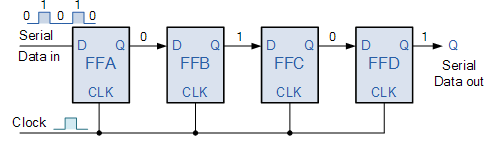
\includegraphics[scale=0.8]{sfr.png}
	\begin{center}
		Fonte: Elaborado pelo Autor
	\end{center}	
\end{figure}

Ao inserir uma realimentação no sistema \textit{shift register}, altera-se a sua entrada e consequentemente os seus estados. A introdução da realimentação gera um sistema LFSR, porém este procedimento deve ser feito de acordo com algumas regras quando deseja-se obter uma determinada propriedade na saída.

Esta realimentação é implementada adicionando portas XOR, juntamente com \textit{flip-flops} como ilustrado na \autoref{model_lfsr}. Cada porta XOR inserida no sistema é denominado de \textit{tap}, definindo um padrão nos dados de saída além de gerar um polinômio característico do LFSR.

\begin{figure}[H]
	\caption{\label{model_lfsr}Tipos de sistemas \textit{Linear Feedback Shift Registers}.}
	\centering
	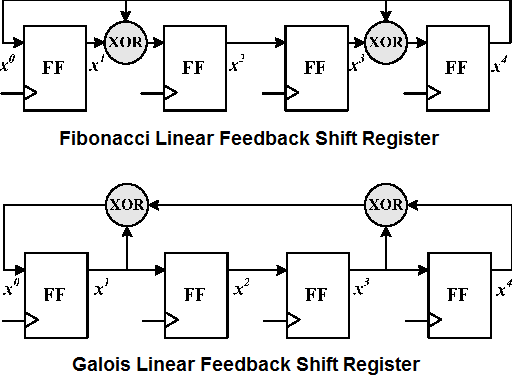
\includegraphics[scale=0.8]{models_lfsr.png}
	\begin{center}
		Fonte: Elaborado pelo Autor
	\end{center}	
\end{figure}

A cada porta XOR inserida no sistema, indica uma expressão matemática ou um polinômio. Cada LFSR possui um padrão na geração dos bits de saída, ou seja, os dados na saída não são puramente aleatórios possuindo um ciclo de repetição. Este padrão é determinado de acordo com o número de estágios e as ligações na realimentação, ou seja, cada esquema (polinômio) implementado possui um padrão no dado da saída. Portanto, a cada ciclo o dado começa a ser repetido e o comprimento deste ciclo é dado por $2^{n} - 1$, em que $n$ é o número de \textit{shift registers} usados no sistema. Porém, para se obter o máximo comprimento no circuito deve-se usar os polinômios primitivos, ou seja, inserir determinados \textit{taps} em  estágios específicos para produzirem o máximo comprimento. 

A teoria de campos finitos é utilizada para definir quando um polinômio é ou não primitivo. No capítulo \ref{primitive:cap} é descrito como obter um polinômio primitivo, ou seja, um polinômio irredutível. Normalmente, estes polinômios são utilizados para construir circuitos geradores de números aleatórios, pelo fato de ocuparem um espaço menor quando comparado com os circuitos desenvolvidos com contadores.

Na tabela da \autoref{maxlfsr} é esboçado alguns polinômios primitivos para 4, 8, 16, e 32 estágios. Observa-se pela tabela que há vários polinômios, ou \textit{taps}, para o mesmo número de \textit{flip flops} porém só há um polinômio primitivo que produz o máximo ciclo no sistema. Estes polinômios são os mesmos para as configurações Fibonacci e Galois. 

\begin{figure}[H]
	\caption{\label{maxlfsr}Tabela de polinômios com máximo comprimento para circuitos LFSR (\textit{shift register}).}
	\centering
	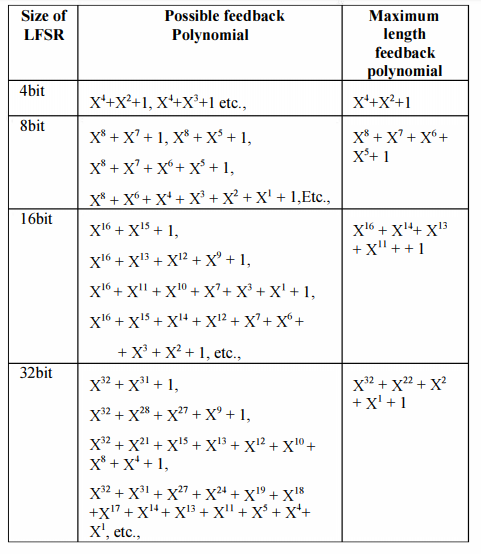
\includegraphics[scale=0.8]{maximal_length_lfsr.png}
	\begin{center}
		Fonte: \cite{Abinaya2014}
	\end{center}	
\end{figure}

Deve-se notar que há algumas regras para a escolha do polinômio primitivo que será implementado pelo circuito LFSR. Estas regras são descritas em \cite{Abinaya2014} e possuem as seguintes características:

\begin{itemize}
	\item O número $1$ descrito nos polinômios da tabela da \autoref{maxlfsr} não correspondem à um \textit{tap} e sim à entrada para o primeiro estágio do sistema.
	\item Os exponentes dos termos do polinômio correspondem aos estágios, e a sua contagem normalmente é feita da esquerda para a direita. Porém, nem todo sistema pode ser montado desta forma. 
	\item Um LFSR só terá comprimento máximo se o número de \textit{taps} for par. Somente 2 ou 4 \textit{taps} pode ser suficiente para gerar longas sequências.
	\item O número do conjunto de \textit{taps}, tomados ao todo, deve ser relativamente primo. Em outras palavras, o polinômio tomado deve ser primitivo.
	\item Depois que um polinômio primitivo for encontrado, outro segue automaticamente. Se os exponentes em um sistema LFSR com $ n $ estágios são da forma [n, A, B, C, 0], onde o 0 corresponde ao termo $1$, então a sequência 'espelho' correspondente é [n, n-C, n-B, n-A, 0]. Assim, com uma sequência igual a [32, 7,3, 2 e 0] pode-se produzir a sua contraparte igual a [32, 30, 29, 25, 0]. Ambos dão uma sequência de comprimento máximo.
\end{itemize}


\section{Fibonacci Linear Feedback Shift Registers}

Um sistema LFSR Fibonacci é uma das formas de criar um LFSR a partir de um \textit{shift register}. A realimentação de sistemas Fibonacci LFSR é caracterizada como externa, uma vez que no caminho da mesma encontra-se portas XOR's. Um esquema da realimentação em circuitos fibonacci é ilustrado na \autoref{fibonacci}

\begin{figure}[H]
	\caption{\label{fibonacci}Esquema de um registrador de deslocamento (\textit{shift register}).}
	\centering
	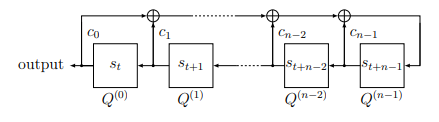
\includegraphics[scale=1.0]{fibonaccilfsr.png}
	\begin{center}
		Fonte: Elaborado pelo Autor
	\end{center}	
\end{figure}

Desta forma, pode-se simplificar a representação de um fibonacci LFSR uma vez que é conhecido a existência de seus estágios e ligações XOR. Uma representação simplificada é ilustrada na \autoref{Simplefibonacci}. Cada estágio é representado pelo símbolo $ S_{j}[k]$ e a ligação entre o estágio e a realimentação, feito por meio de portas XOR's, é representado por $b_{j}$ o qual pode ser $0$ ou $1$. O $j$ especifica o estágio e o $k$ o período que está sendo referido.

\begin{figure}[H]
	\caption{\label{Simplefibonacci}Esquema de um sistema (\textit{Fibonacci Linear Feedback Shift Register}).}
	\centering
	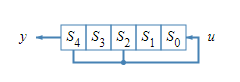
\includegraphics[scale=1.0]{fibonaccilfsr_simple.png}
	\begin{center}
		Fonte: Elaborado pelo Autor
	\end{center}	
\end{figure}

A entrada do sistema representado na \autoref{Simplefibonacci} pode ser definido pela expressão matemática:

$$ u[k] = \bigoplus_{j = 0}^{N - 1} b_{j}S_{j}[k] $$

O símbolo $ \bigoplus $ significa uma operação XOR com todas as entradas no mesmo tempo. Desta forma, na \autoref{Simplefibonacci} as variáveis $ b_{j} $ são definidas como: $ b_{2} = b_{4} = 1 $ e $ b_{0} = b_{3} = b_{0} = b_{1} = 0 $. Portanto, a equação da entrada é definida como $ u[k] = S_{4}[k] \bigoplus S_{2}[k] = u[k-5] \bigoplus u[k-3] $ e a saída é simplesmente a entrada atrasada o número de estágios no LFSR, ou seja, neste caso a saída é atrasada 5 períodos obtendo a equação $y[k] = u[k-5] = y[k-5] \bigoplus y[k-3] $. 

\section{Galois Linear Feedback Shift Registers}

O outro tipo de sistema que pode ser construído realimentando um \textit{shift register} é o Galois LFSR. A realimentação destes sistemas é caracterizada como interna, uma vez que as portas XOR's estão no caminho entre os \textit{flips flops} ao invés de estarem na realimentação. Um esquema de circuitos Galois LFSR é ilustrado na \autoref{galois_lfsr}

\begin{figure}[H]
	\caption{\label{galois_lfsr}Esquema de um sistema (\textit{Galois Linear Feedback Shift Register}).}
	\centering
	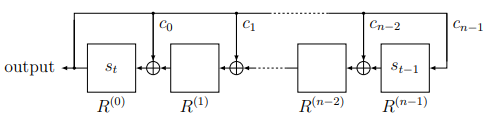
\includegraphics[scale=1.0]{galoislfsr.png}
	\begin{center}
		Fonte: Elaborado pelo Autor
	\end{center}	
\end{figure}

Desta forma, pode-se simplificar a representação de um Galois LFSR uma vez que é conhecido a existência de seus estágios e ligações XOR. Uma representação simplificada é ilustrada na \autoref{Simplegalois}. Cada estágio é representado pelo símbolo $ S_{j}[k]$ e a ligação entre o estágio e a realimentação, feito por meio de portas XOR's, é representado por $a_{j}$ o qual pode ser $0$ ou $1$. O $j$ especifica o estágio e o $k$ em qual período está sendo referido.

\begin{figure}[H]
	\caption{\label{Simplegalois}Esquema simplificado de um sistema (\textit{Galois Linear Feedback Shift Register}).}
	\centering
	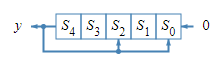
\includegraphics[scale=1.0]{galoislfsr_simple.png}
	\begin{center}
		Fonte: Elaborado pelo Autor
	\end{center}	
\end{figure}

Na representação de Galois de um LFSR, a entrada $u$ é setada para $0$ mas somente os estágios que possuem uma porta XOR ligada na saída podem alterar os bits transmitidos. Portanto, a saída $y[k]$ do LFSR  representado na \autoref{Simplegalois} pode ser definida como:

$$ S_{j}[k] = S_{j-1}[k-1] \bigoplus a_{j}y[k-1] \quad para \quad j \quad > \quad 0 $$
$$ S_{0}[k] = a_{0}y[k-1] $$
$$ y[k] = S_{N-1}[k] \quad N: \quad número \quad de \quad estágios$$ 

Desta forma, na \autoref{Simplegalois} as variáveis $ a_{j} $ são definidas como: $ a_{0} = a_{2} = 1 $ e $ a_{1} = b_{3} = b_{4} = 0 $. Portanto, a equação dos estágios e da saída são definidas da forma:

$$ S_{0}[k] = y[k-1]  $$
$$ S_{1}[k] = S_{0}[k-1] = y[k-2]  $$
$$ S_{2}[k] = S_{1}[k-1] \bigoplus y[k-1] = y[k-3] \bigoplus y[k-1] $$
$$ S_{3}[k] = S_{2}[k-1]  =  y[k-4] \bigoplus y[k-2] $$
$$ S_{4}[k] = S_{3}[k-1]  =  y[k-5] \bigoplus y[k-3] $$
$$ y[k] = S_{4}[k] = y[k-5] \bigoplus y[k-3] $$

Na configuração de Galois os estágios que não possuem \textit{taps} conectados, são deslocados uma posição para o próximo estágio. Os \textit{taps}, por outro lado, realizam uma operação XOR com o bit de saída do estágio antes de serem armazenados na próximo \textit{flip-flop}.O efeito disto é que quando o bit de saída é zero, todos os bits no registrador mudam para a direita inalterados, e o bit de entrada se torna zero. Quando o bit de saída é um, os bits nas posições da derivação são invertidos (se forem 0, eles se tornarão 1, e se forem 1, eles se tornarão 0). Desta forma, o registrador inteiro será deslocado para a direita e o bit de entrada torna-se 1.

Um Fibonacci LFSR, na presença de muitos taps, opera em velocidades mais baixas quando comparado com os sistemas Galois LFSR. Isto ocorre pelo fato das diversas portas XOR no caminho da realimentação ocasionarem um \textit{delay} maior do que somente uma porta entre cada estágio descrito nos sistemas Galois LFSR. Porém, sistemas Fibonacci LFSR podem operar em velocidades altas como os Galois, se  existir no máximo uma porta XOR no caminho da realimentação \cite{Sachin2018}.

\chapter[Scramblers]{Scramblers} \label{teo:scrambler}

Em sistemas de comunicação, um \textit{scrambler} é um dispositivo que consegue embaralhar ou modificar uma mensagem no lado do emissor para tornar a mensagem ininteligível ou com determinadas propriedades para o receptor que não possui a capacidade de interpretar aquela mensagem. O embaralhamento é realizado pela adição ou reordenamento de componentes ao sinal original a fim de dificultar a extração do mesmo. Alguns \textit{scramblers} modernos são, na verdade, dispositivos de criptografia, permanecendo o nome devido às semelhanças no uso, em oposição à operação interna \cite{Ghassan2018}.

Nas comunicações digitais, em muitos casos, um \textit{scrambler} é usado para manipular um fluxo de dados antes de transmitir. As manipulações são invertidas por um \textit{descrambler} no lado de recepção. Estas manipulações tem o objetivo de embaralhar o dado a ser transmitido, porém pode não haver criptografia neste processo. A intenção nesse caso não é tornar a mensagem ininteligível, mas dar aos dados transmitidos propriedades de engenharia úteis \cite{Ghassan2018}. Estas propriedades são úteis para a codificação 64b/66b.

Estas propriedades podem serem resumidas em dua principais \cite{Ghassan2018}:

\begin{itemize}
	\item O embaralhamento em sistemas de comunicação digital facilita a atuação dos circuitos de recuperação de \textit{clock}, controle de ganho e outros circuitos adaptativos do receptor pela eliminação de sequências consistindo apenas de $0's$ ou $1's$.
	\item Um circuito \textit{scrambler} torna o espectro de potência do sinal mais disperso para atender ao requisitos de densidade espectral de potência. Este requisito trata da potência concentrada em uma faixa de frequência estreita, uma vez que esta característica pode interferir canais devido à modulação cruzada e à intermodulação causada 	pela não linearidade do receptor.
\end{itemize}

Os \textit{scramblers} usualmente são definidos com base em LFSR por conta de suas boas características estatísticas, bem como pela facilidade de implementação em hardware. Os \textit{scramblers} podem serem separados em dois tipos: \textit{Scramblers} Aditivos (Synchronous) e Multiplicativos (Self-Synchronizing).

\section{\textit{Scramblers} Aditivos (Synchronous)}

\textit{Scramblers} Aditivos transformam o fluxo de dados de entrada, aplicando uma sequência binária pseudoaleatória (PRBS) por adição módulo-2. Em alguns casos, um PRBS pré-calculado é armazenado em uma memória ROM, sendo usado quando necessário. Entretanto, frequentemente é gerado por um LFSR devidamente implementado no sistema. Um esquema de um \textit{scrambler} aditivo é ilustrado na \autoref{additive_scrambler}.

\begin{figure}[H]
	\caption{\label{additive_scrambler}Esquema de um \textit{Scramblers} Aditivo.}
	\centering
	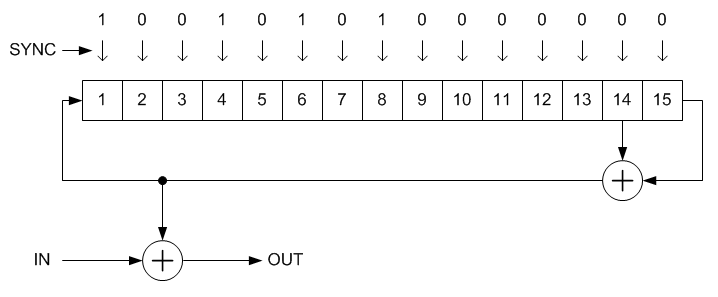
\includegraphics[scale=0.6]{Scrambler_randomizer_additive.png}
	\begin{center}
		Fonte: Elaborado pelo Autor
	\end{center}	
\end{figure}

Uma palavra de sincronização é usada para assegurar uma operação síncrona do LFSR. Esta palavra é um padrão inserido no fluxo de dados em intervalos de tempos iguais, como por exemplo logo após o tempo para processar o dado introduzido no circuito. Um receptor procura algumas palavras de sincronização em dados adjacentes e, portanto, determina o local em que seu LFSR deve ser recarregado com um estado inicial predefinido \cite{Ghassan2018}.

O \textit{descrambler} aditivo é apenas o mesmo dispositivo que o \textit{scrambler} aditivo. O \textit{scrambler} /  \textit{descrambler} aditivo são definidos pelo polinômio de seu LFSR e seu estado inicial.

\section{\textit{Scramblers} Multiplicativos (Self-Synchronizing)} \label{scrambler_multi}

Os \textit{scramblers} multiplicativos são chamados assim por executarem uma multiplicação do sinal de entrada pela função de transferência do \textit{scrambler} no espaço Z. Eles são sistemas lineares invariantes no tempo. Ao contrário dos \textit{scramblers} aditivos, os \textit{scramblers} multiplicativos não precisam da palavra sincronização, por isso eles também são chamados de auto-sincronizadores.  Um exemplo da topologia dos \textit{scramblers} multiplicativos está representado na \autoref{multiplicative_scrambler}. Na letra (a) é representado um \textit{scrambler} e na letra (b) um \textit{descrambler} \cite{Ghassan2018}.

\begin{figure}[H]
	\caption{\label{multiplicative_scrambler}Esquema de um \textit{Scramblers} Multiplicativo.}
	\centering
	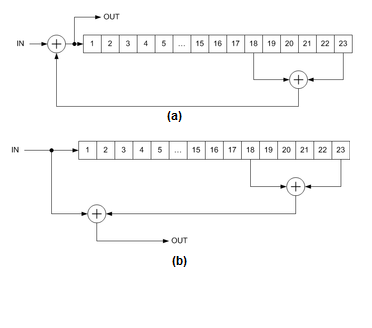
\includegraphics[scale=1.2]{Scrambler_randomizer_multiplicative.png}
	\begin{center}
		Fonte: Elaborado pelo Autor
	\end{center}	
\end{figure}

\textit{Scrambler} multiplicativo é definido similarmente por um polinômio, que também é uma função de transferência do \textit{descrambler}. A saída codificada, $S(x)$, é gerada no transmissor dividindo os dados $M(x)$ por um polinômio gerador $G(x)$:

$$S(x) = \dfrac{M(x)}{G(x)}$$

A operação de divisão é realizada bit a bit e cada etapa da divisão resulta em um novo bit embaralhado. O receptor reordena o sinal embaralhado multiplicando pelo mesmo polinômio gerador:

$$M(x) = S(x)*G(x)$$

A implementação da divisão e multiplicação polinomial é feita usando \textit{Linear feedback shift registers}, além de toda a teoria de campos finitos e suas operações em módulo 2. 

Os embaralhadores multiplicativos levam à multiplicação de erros durante a descodificação. Um erro de bit único na entrada do descodificador resultará em $w$ erros na sua saída. Este aumento no número de erros depende do número de \textit{taps} existente no sistema. Caso existir duas \textit{taps}, um único bit de erro inserido no sistema resultará em 3 bits errôneos na saída do \textit{descrambler} \cite{Ghassan2018}. 

\chapter[CRC]{Cyclic Redundancy Check (CRC)} \label{crc:teoria}

Um CRC é um algorítimo somador para detectar erros durante a transmissão dos dados. Dado um bloco de com k bits, o CRC produz r bits que são adicionados ao bloco original e sendo transmitidos pelo meio de comunicação. O adendo r é uma constante e normalmente está entre 8 e 32 bits, para implementações reais. Portanto a mensagem final possui $n = k + r$ bits, gerados pela soma dos k bits do bloco mais o adendo gerado pelo CRC. Um exemplo de um CRC genérico é ilustrado na \autoref{example_crc}.

\begin{figure}[H]
	\caption{\label{example_crc}Exemplo genérico de um sistema CRC.}
	\centering
	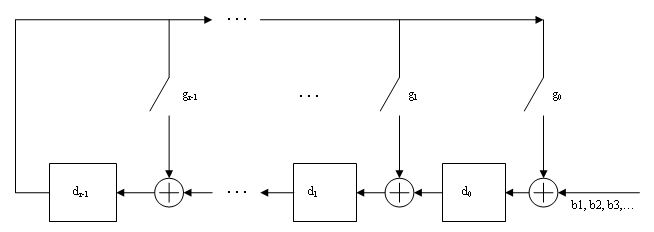
\includegraphics[scale=0.8]{example_crc.png}
	\begin{center}
		Fonte: Elaborado pelo Autor
	\end{center}	

\end{figure}

Cada mensagem final possui uma distância mínima de Hamming para auxiliar na detecção de erros. A distância de Hamming significa que a partir daquele número de bits errôneos no dado transmitido o sistema não consegue detectar. Para o mesmo circuito CRC pode-se obter diferentes distâncias de Hamming, dependendo do número $k$ de bits do dado a ser transmitido \cite{Tridib2004}.	

Um CRC é um exemplo de um código polinomial, bem como um exemplo de um código cíclico. A ideia em um código polinomial é representar cada bloco de códigos $w = w_{n − 1} w_{n − 2} w_{n − 2} w_{0}$ como um polinômio de grau $(n - 1)$. Portanto, tem-se:

$$ w(x)= \sum_{i = 0}^{n - 1} w_{i}x^{i}$$

O propósito no sistema CRC é garantir que todo polinômio $w(x)$ seja múltiplo de um polinômio gerador, $g(x)$. Toda aritmética no CRC será feita por meio dos campo finitos com 
operações em módulo-2. As regras normais de adição polinomial, divisão e multiplicação são aplicáveis, exceto quando todos os coeficientes são $0$ ou $1$ \cite{Tridib2004}.

\section{Codificação do Dado}
Para que $w(x)$ seja múltiplo de $g(x)$ deve-se obter $w(x)$ por meio do dado de entrada $m(x)$ e $g(x)$, de modo que $g(x)$ divida $w(x)$. Deve-se multiplicar $m(x)$ por $x^{n − k}$. Desta forma o dado de entrada é deslocado $(n  k)$ bits, então pode-se adicionar os bits produzidos pelo CRC. Após deslocar o dado de entrada em $n - k$ bits, nos espaços vagos são inseridos bits $0's$. Portanto, o dado final com os bits $0's$ inseridos nos espaços vagos é representado por: $x^{n − k}m(x)$ \cite{Tridib2004}.

Posteriormente, divide-se o dado deslocado $x^{n − k}m(x)$, por $g(x)$. Se o restante da divisão polinomial é 0, portanto os bits adicionados no espaço vagos estão corretos. Caso contrário, temos um resto, $R$. Ao subtrair este resto $R$ do polinômio $x^{n - k}m(x)$, obtêm-se um novo polinomial que será um múltiplo de $g(x)$. Como a subtração é feita no campo finito $GF(2)$, pode-se substituir a subtração pela soma em $GF(2)$, obtendo-se:

$$ w(x) = x^{n − k}m(x) + R{\dfrac{x^{n−k}m(x)}{g(x)}} $$

Um exemplo desta operação está ilustrada na \autoref{encoding_crc}. A mensagem é definida como $m(x) = 1101011011$ e o polinômio gerador do CRC é definido como $g(x) = 10011$. Deve-se salientar que foi usado a divisão longa no campo finito $GF(2)$.

\begin{figure}[H]
	\caption{\label{encoding_crc}Procedimento da codificação para o sistema CRC.}
	\centering
	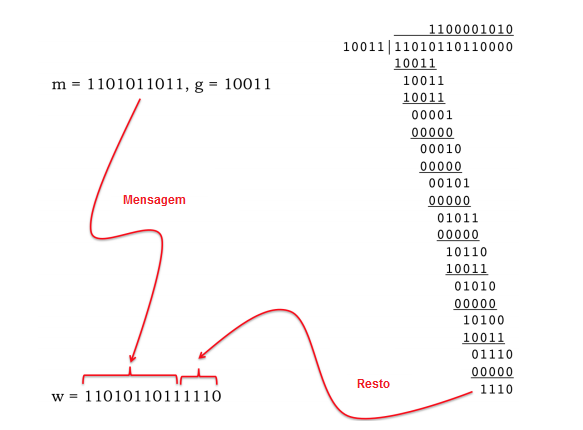
\includegraphics[scale=1.0]{encoding_crc.png}
	\begin{center}
		Fonte: Elaborado pelo Autor
	\end{center}	
\end{figure}

O $R{(\dfrac{x^{n−k}m(x)}{g(x)})}$ refere-se para o resto da divisão de $x^{n − k}m(x)$ por $g(x)$. Portanto, $w(x)$ é a mensagem final com $n = k + r$ bits que será transmitida pelo canal de comunicação \cite{Tridib2004}.

\section{Decodificação do Dado}

A etapa de decodificação é idêntica à etapa de codificação, além do decodificador possuir o mesmo polinômio gerador $g(x)$ do codificador. Nesta etapa, separa-se o dado $x^{n − k}m(x)$ do resto do CRC, adicionando $0's$ no lugar do resto. Posteriormente, verifica-se o resto calculado pela divisão de $x^{n − k}m(x)$ recebido por $g(x)$, comparando com o resto recebido no decodificador. Uma incompatibilidade entre os dois restos garante que ocorreu um erro \cite{Tridib2004}.

\section{Seleção de Polinômios Geradores} \label{poli:gerador}

Normalmente nas transmissões ocorre padrões de erro para os dados recebidos, desta forma pode-se formar algumas ideias na escolha do polinômio. Para desenvolver propriedades adequadas para $g(x)$, deve-se obter o polinômio $r(x)$ que é a soma do dado enviado $w(x)$ e um erro polinomial $e(x)$ \cite{Tridib2004}.

Se $r(x) = w(x) + e(x)$ não é um múltiplo de $g(x)$, então o receptor certamente detectará o erro. O dado $w(x)$ é construído como um múltiplo de $g(x)$, se $e(x)$ não é um múltiplo de $g(x)$, o receptor detectará o erro. Por outro lado, se $r(x)$ e, portanto, $e(x)$, é um múltiplo de $g(x)$, então o erro não é detectado. Deve-se garantir que esta situação não ocorra para erros que ocorrem com frequência na transmissão \cite{Tridib2004}
. Portanto, pode-se seguir a seguinte instruções:

\begin{itemize}
	\item Para padrões de erro únicos, $e(x) = x^{i}$ para alguns $i$. Isso significa que devemos assegurar que $g(x)$ tenha pelo menos dois termos.
	\item Para detectar todos erros duplos (ou pares) acontecidos na transmissão, pode-se representar este padrão de erro como $x^{i} + x^{j} = x^{i}(1 + x^{j − i})$, para alguns $i$ e $j > i$. Se $g(x)$ não for múltiplo deste termo, então o CRC pode detectar todos os erros duplos.
	\item Para detectar todos os números ímpares de erros, deve-se ter um $g(x)$ que possua um número par de termos e que $(1 + x)$ seja um fator de $g(x)$. A divisão de qualquer polinômio no campo finito $GF(2)$ da forma $(1 + x)h(x)$ é avaliado como $0$ quando setamos $x$ para $1$. Ao expandir $(1 + x)h(x)$ deve possuir um número par de termos. Portanto, se $(1 + x)$ for um fator de $g(x)$, o CRC será capaz de detectar todos os padrões de número ímpar de erros. No entanto, a inversa não é verdadeira: um CRC pode detectar um número ímpar de erros mesmo quando o seu $g(x)$ não é um múltiplo de $(1 + x)$. Porém, todos os CRC's usados na prática	possuem $(1 + x)$ como um fator de $g(x)$ porque é a maneira mais simples de atingir esse objetivo.
	\item Para detectar rajada de erros, primeiramente define-se um o padrão do erro de rajada com comprimento $b$ como uma sequência de bits $1\varepsilon_{b} − 2\varepsilon_{b − 3} ... \varepsilon_{1}1$.  O número de bits é $b$, o primeiro e o último bits são ambos 1, e os bits $\varepsilon_{i}$ no meio podem ser $0$ ou $1$. O comprimento mínimo da rajada é $2$, correspondente ao padrão “11”. 

	Para o CRC detectar todos esses padrões de erros, primeiro define-se o padrão de erros de rajada como $e(x)=	x^{s} (1 * x^{b-1} + \sum_{i = 1}^{b − 2} \varepsilon_{i}x^{i} + 1)$. Este polinômio possui tamanho $b$ e começa com $s$ bits à esquerda no final do pacote. Se escolher-se $g(x)$ para ser um polinômio de grau $b$, e se $g(x)$ não tem $x$ como um fator, então qualquer padrão de erro com comprimento $\leq b$ pode ser detectado. Isto deve-se ao fato de $g(x)$ não dividir um polinômio de grau menor que o seu. Além disso, existe um padrão de erro de comprimento $b + 1$ que corresponde quando o padrão de erro de rajada iguala-se aos coeficientes do próprio $g(x)$. Quando essa condição é atingida não pode-se detectar erros no dado recebido. Caso contrário, todos os outros padrões de erro de comprimento $b + 1$ serão detectados pelo CRC.
\end{itemize}


\section{Implementação em Hardware}

O fluxo de dados de entrada no CRC é geralmente bastante longo, sendo normalmente mais de 1 bit. Portanto não é possível executar uma divisão simples. A computação deve ser executada passo a passo, desta forma um \textit{shift register} é utilizado.

Um \textit{shift register} possui um comprimento fixo, sendo possível o deslocamento de bits no seu interior. Portanto, é possível remover o bit na borda direita ou esquerda e deslocar outro bit na posição liberada. O CRC usa um \textit{shift register} que desloca dados da posição menos significativa (LSB) para a mais significativa (MSB). A posição do bit menos significativo é de livre escolha.

O processo de cálculo do CRC usando um \textit{shift register} é o seguinte:

\begin{itemize}
	\item Inicializar todos os \textit{shift register} com o bit $0$.
	\item Desloca-se o primeiro bit do dado de entrada dentro do sistema. Quando o bit MSB que sair do sistema for um '1', realiza-se uma operação XOR com o valor de todos os \textit{shift registers} (contanto com o bit MSB que foi deslocado) com o polinômio do gerador. O resultado é inserido nos registradores e continua a operação.
	\item Se todos os bits de entrada forem inseridos, os \textit{shift registers} do CRC contém o valor de CRC que será adicionado ao dado.
\end{itemize}

Para implementações em software o sistema pode ser implementado descrevendo em código o LFSR do CRC desenvolvido, usando a técnica bit a bit. Porém, na literatura há várias implementações em software mais que calculam o resultado do CRC de forma mais rápida do que realizar bit a bit.
